\documentclass[12pt]{article}
\usepackage{xeCJK}%preamble part
\usepackage{graphicx}
\usepackage{indentfirst}
\usepackage[a4paper, inner=1.5cm, outer=3cm, top=2cm, bottom=3cm, bindingoffset=1cm]{geometry}
\usepackage{epstopdf}
\usepackage{listings}
\usepackage{array}
\usepackage{fontspec}
\usepackage{bm}
\usepackage{gensymb}
\usepackage{todonotes}
\usepackage{amsmath, amsthm, amssymb}
\usepackage[citecolor=blue]{hyperref}
\newtheorem{definition}{Definition}
\newtheorem{thm}{Theorem}[section]
\newtheorem{cor}[thm]{Corollary}
\newtheorem{lem}[thm]{Lemma}
\DeclareMathOperator{\sgn}{sgn}
\theoremstyle{remark}
\newtheorem*{rem}{Remark}
\usepackage{makecell}
\usepackage[lofdepth,lotdepth]{subfig}




\setlength{\extrarowheight}{4pt}
\setlength{\parindent}{1cm}
\begin{document}
\title{\textbf{\fontsize{15.75pt}{\baselineskip}{讨论}}} 

\author{\fontsize{12pt}{\baselineskip}{数33 赵丰}}
\maketitle
\large
本次讨论在2移动节点协作的场景下从两种角度给出方位角的最优部署,并尝试将global optimization推广至多节点协作的情形。
根据前面对符号的约定,可以从read6.pdf中(19)式出发求移动节点1的SPEB为:
\begin{equation}
\text{SPEB}=\text{tr}(\text{FIM}^{-1})
\end{equation}
这里FIM的表达式为:
\begin{equation}
\text{FIM}=\bm{\Sigma}_0+\xi_{1,2}\epsilon\bm{u}\bm{u}^T
\end{equation}•
其中$\bm{\Sigma}_0=\text{diag}\{\lambda_1,\lambda_2\},\bm{u}$是方向角为$\theta$的方向向量,而$\xi_{1,2}$是EFII,为:
\begin{equation}
\xi_{1,2}=\frac{1}{1+\epsilon \bm{v}\bm{\Sigma}_1^{-1}\bm{v}}
\end{equation}
上式中$\bm{v}$是方向角为$\phi$的方向向量,而$\bm{\Sigma}_1=\text{diag}\{\lambda_3,\lambda_4\}$
根据之前的公式:
\begin{equation}
\text{SPEB}=\frac{1}{\xi_1}+\frac{1}{\xi_2}
\end{equation}
其中$\xi_1,\xi_2$是FIM的特征值:
因此考虑求|FIM|,由上一节的公式:
\begin{equation}
|\text{FIM}|=(\lambda-\lambda_1)(\lambda-\lambda_2)-\xi_{1,2}\epsilon(\cos^2(\theta)(\lambda-\lambda_2)+\sin^2(\theta)(\lambda-\lambda_1))
\end{equation}
利用根与系数的关系可求出:
\begin{equation}
\text{SPEB}=\frac{\lambda_1+\lambda_2+\xi_{1,2}\epsilon}{\lambda_1\lambda_2+\xi_{1,2}\epsilon(\cos^2(\theta)\lambda_2+\sin^2(\theta)\lambda_1)}
\end{equation}
这个式子和讨论非协作定位时推导的SPEB是相通的,如果把
$\xi_{1,2}\epsilon$当成一个整体,那么与沈老师文献I中(21)式相同,在已知RII极小化SPEB过程中,只需先处理$\xi{1,2}$,确定$\phi$,再用之前的结论确定$\theta$即可。分析如下:
由于考虑了协作,SPEB比非协作的情形$\frac{\lambda_1+\lambda_2}{\lambda_1\lambda_2}$减小了一些,二者作差有:
\begin{equation}\label{eq:Delta}
\Delta=\frac{\lambda_1+\lambda_2}{\lambda_1\lambda_2}-\text{SPEB}=\xi(\frac{\cos^2(\theta)}{\lambda_1^2}+\frac{\sin^2(\theta)}{\lambda_2^2})
\end{equation}
其中
\begin{equation}
\xi=1/(\frac{1}{\epsilon}+\frac{\cos^2(\phi)}{\lambda_3}+\frac{\sin^2(\phi)}{\lambda_4}+\frac{\cos^2(\theta)}{\lambda_1}+\frac{\sin^2(\theta)}{\lambda_2})
\end{equation}
为使SPEB最小,$\Delta$应最大。先极大化$\xi$求出$\phi=0$(设$\lambda_3>\lambda_4$),这个方向是节点2非协作的信息椭圆短轴所在的直线方向,给定$\phi=0$后,极大化$\Delta$有$\theta=\frac{\pi}{2}$,即沿节点1非协作的信息椭圆短轴所在的直线方向而沿节点2非协作的信息椭圆长轴所在的直线方向(取长补短)。因此在极值条件下两个移动节点的信息椭圆的位置应如下图所示:
%原来的图画错了!
\begin{figure}[!ht]
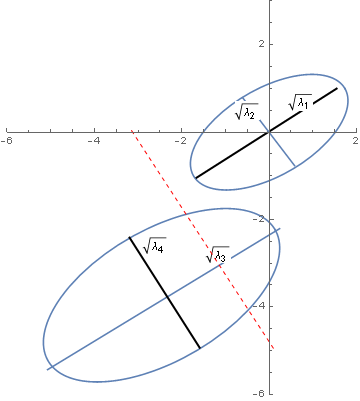
\includegraphics[width=\textwidth]{InfoEllipse.png}
\end{figure}•

这个结论下无法做到全局最优,因为一旦取节点2的长补节点1的短,那么由于两节点之间方向不能改变,节点2本身的短不能用节点1的长来补(这个方向和前面的方向垂直),所以这个结论是不对称的,是以牺牲另一个节点的定位精度来满足目标节点的需求。
%说明使得两个移动节点定位误差分别最小的部署方案满足两个条件:
%\begin{enumerate}
%\item{非协作情形下两个移动节点的信息椭圆方向一致}
%\item{增加协作时要求两个移动节点位置的连线与非协作信息椭圆短半轴所在直线共线}
%\end{enumerate}

此时$\Delta_{\text{max}}=\frac{1\lambda_2^2}{1/\epsilon+1\lambda_4+1/\lambda_2}$.表示协作使SPEB下降的成分。$\Delta_{\text{max}}$随$\lambda_4,\epsilon$增加而增加,但随$\lambda_2$增加而减小,说明如果节点1本身信息量比较大($\lambda_2$大),那么节点2对节点1定位的贡献会小。

下面我们给出使得两个节点SPEB最小的部署方案:

由之前的讨论,SPEB等于高维信息椭圆特征值的倒数和,对于n阶方程$|\lambda \bm{I}-A|=0$,通过提取$\lambda^n$变成关于$\eta=\frac{1}{\lambda}$的n阶方程,通过根与系数的关系可表示出SPEB.

对于上节给出的4维矩阵A,整理得到:
\[
\text{SPEB}_{\text{global}}=
\]
\begin{equation}\label{eq:SPEB_GLOBAL}
\begin{split}
\frac{\displaystyle\sum \frac{1}{\lambda_i}+\epsilon(\frac{\cos^2(\theta)}{\lambda_1}(\sum_{i \neq 1}\frac{1}{\lambda_i})+\frac{\sin^2(\theta)}{\lambda_2}(\displaystyle\sum_{i \neq 2}\frac{1}{\lambda_i})+\frac{\cos^2(\phi)}{\lambda_3}(\sum_{i \neq 3}\frac{1}{\lambda_i})+\frac{\sin^2(\phi)}{\lambda_4}(\sum_{i \neq 4}\frac{1}{\lambda_i}))}{\displaystyle 1+\epsilon(\frac{\cos^2(\theta)}{\lambda_1}+\frac{\sin^2(\theta)}{\lambda_2}+\frac{\cos^2(\phi)}{\lambda_3}+\frac{\sin^2(\phi)}{\lambda_4})}
\end{split}
\end{equation}
观察上式,SPEB对$\theta$和$\phi$的依赖是通过正余弦函数的平方给出的,再考虑对于固定的$\theta$或$\phi$,SPEB关于另一个变量是单调递减的,即极值只能在$[0,\frac{\pi}{2}]\times[0,\frac{\pi}{2}]$正方形四个角点取到。不失一般性设$\lambda_1>\lambda_2$,$\lambda_3>\lambda_4$,我们试图寻找正方形的右上角点$\theta=\phi=\frac{\pi}{2}$是使得SPEB最小的角点的一个必要条件。在这个必要条件下如果这个结论成立,那么两节点协作方向全局最优解是短(轴)对短(轴)。
\begin{thm}
如果$\frac{1}{\lambda_1}+\frac{1}{\lambda_2}\geq\frac{1}{\lambda_4}$且$\frac{1}{\lambda_3}+\frac{1}{\lambda_4}\geq\frac{1}{\lambda_2}$,那么$\theta=\phi=\frac{\pi}{2}$是$(\ref{eq:SPEB_GLOBAL})$的最小值点。
\end{thm}
\begin{proof}
对固定的$\phi$,我们证明SPEB关于$\theta$是单调递减的。记$k=\frac{\cos^2 \theta}{\lambda_1}+\frac{\sin^2 \theta}{\lambda_2}$,$u=(\frac{1}{\lambda_3}+\frac{1}{\lambda_4}),v=(\frac{1}{\lambda_1}+\frac{1}{\lambda_2})$(\ref{eq:SPEB_GLOBAL})可以化为:
\begin{equation}
\text{SPEB}=u\frac{1+(\frac{1}{\lambda_1}+\frac{1}{\lambda_2})/u+\epsilon(\frac{1}{\lambda_1\lambda_2 u}+\frac{1}{\lambda_3\lambda_4 u}+k+(\frac{\cos^2\phi}{\lambda_3}+\frac{\sin^2\phi}{\lambda_4})\frac{v}{u})}{1+\epsilon(k+(\frac{\cos^2\phi}{\lambda_3}+\frac{\sin^2\phi}{\lambda_4}))}
\end{equation}
SPEB可以写成关于k的反比例函数$u\frac{A+k}{B+k}$的形式,其中
\[
A=(1+(\frac{1}{\lambda_1}+\frac{1}{\lambda_2})/u)/\epsilon+\frac{1}{\lambda_1\lambda_2 u}+\frac{1}{\lambda_3\lambda_4 u}+(\frac{\cos^2\phi}{\lambda_3}+\frac{\sin^2\phi}{\lambda_4})\frac{v}{u}
\]
\[
B=1/\epsilon+(\frac{\cos^2\phi}{\lambda_3}+\frac{\sin^2\phi}{\lambda_4})
\]
如果能证明$A \geq B$,那么该反比例函数关于k是单调递减的。
\[
A-B=(\frac{1}{\lambda_1}+\frac{1}{\lambda_2})/u\epsilon+\frac{1}{\lambda_1\lambda_2 u}+\frac{1}{\lambda_3\lambda_4 u}+(\frac{\cos^2\phi}{\lambda_3}+\frac{\sin^2\phi}{\lambda_4})(\frac{v}{u}-1)
\]
\[
\geq \frac{1}{\lambda_3\lambda_4 u}+(\frac{\cos^2\phi}{\lambda_3}+\frac{\sin^2\phi}{\lambda_4})(\frac{v}{u}-1)
\]
\[
=\frac{1}{u}((\frac{1}{\lambda_1}+\frac{1}{\lambda_2})(\frac{\cos^2\phi}{\lambda_3}+\frac{\sin^2\phi}{\lambda_4})-(\frac{\cos^2\phi}{\lambda_3^2}+\frac{\sin^2\phi}{\lambda_4^2}))
\]
由假设:$\frac{1}{\lambda_1}+\frac{1}{\lambda_2}\geq\frac{1}{\lambda_4}\geq \frac{1}{\lambda_3}$
所以$A-B\geq 0$。
下面再证明k关于$\sin^2(\theta)$是单调递增的,那么由复合函数的单调性的性质,结论成立。
\[
k=\frac{1}{\lambda_1}+\sin^2 \theta(\frac{1}{\lambda_2}-\frac{1}{\lambda_1})
\]
因为$\lambda_1\geq \lambda_2$所以在$\sin^2(\theta)\in[0,1]$的区间内结论成立。
同理可证明条件$\frac{1}{\lambda_3}+\frac{1}{\lambda_4}\geq\frac{1}{\lambda_2}$是保证固定$\theta$的情况下SPEB关于$\phi \in [0,\frac{\pi}{2}]$是单调递减的。
\end{proof}
比较SPEB相较于非协作的情形降低的幅度有:
\begin{equation}
\Delta=\sum \frac{1}{\lambda_i}-\text{SPEB}_{\text{global}}=\frac{1}{\xi}(\frac{\cos^2(\theta)}{\lambda_1^2}+\frac{\sin^2(\theta)}{\lambda_2^2}+\frac{\cos^2(\phi)}{\lambda_3^2}+\frac{\sin^2(\phi)}{\lambda_4^2})
\end{equation}
其中$\xi$在(\ref{eq:Delta})式已经定义过了,
与(\ref{eq:Delta})式比较发现全局降低的幅度为单独考虑每个节点单独考虑误差下界降低幅度之和,这从矩阵的迹的角度很容易理解。从全局考虑,在前面定理的假设下最小值正方形的右上角点取到,而单独考虑只能取到正方形左上或右下角点。
%但具体的单调性如何和$\lambda$以及另一个角度这些参数有关,为便于分析又不失一般性,假设非协作的信息椭圆都是圆(在之前讨论中分析了圆是SPEB最小的部署方式,且只需调整2个锚点的部署即可达到最优,在之后讨论多个移动节点的情形,我们总假定非协作总是以最优的姿态出现).在圆的假定下,$\lambda_1=\lambda_2,\lambda_3=\lambda_4$,$\theta \equiv \phi$在(\ref{eq:Delta})式子中,$\Delta$不依赖于

%都是常数,无法讨论。
第一篇翻译
推导:
\begin{equation}
\check{\zeta_{1,2}}=\zeta_{1,2} \cdot \Phi_{1,2}(\bm{J}_2^{\mathcal{N}_b}+\zeta_{2,3} \cdot \Phi_{2,3}(\bm{K}_3^{1})\cdot \bm{C}_{2,3})
\end{equation}•
由EFIM可知
\begin{equation}
\bm{J}_1=\bm{K}_1^{2,3}-(\zeta_{1,2}\bm{C}_{1,2},\zeta_{1,3}\bm{C}_{1,3})\left(
\begin{array}{cc}
\bm{K}_2^{1,3} & -\zeta_{2,3}\bm{C}_{2,3}\\
-\zeta_{2,3}\bm{C}_{2,3} & \bm{K}_3^{1,2}\\
\end{array}
\right)^{-1}\binom{\zeta_{1,2}\bm{C}_{1,2}}{\zeta_{1,3}\bm{C}_{1,3}}
\end{equation}
考虑到一般的情形中对给定的两个二元向量$\bm{u},\bm{v}$(比如(1,0)和(0,1)),四个矩阵$\bm{u}\bm{v}^T,\bm{v}\bm{u}^T,\bm{u}\bm{u}^T,\bm{v}\bm{v}^T$张成2乘2矩阵的一组基,因此$\bm{J}_1-\bm{J}_1^{\mathcal{N}_b}$在由$\bm{u}_{1,2},\bm{u}_{1,3}$张成的基底下的系数可以唯一的确定,通过分离变量可以知道$\bm{u}_{1,2}\bm{u}_{1,2}^T$的系数为
\begin{equation}
\check{\zeta}_{1,2}=\zeta_{1,2}(1-\zeta_{1,2}\bm{u}_{1,2}^T(\bm{K}_2^{1,3}-\zeta^2_{2,3}\bm{C}_{2,3}
(\bm{K}_3^{1,2})^{-1}\bm{C}_{2,3})^{-1}\bm{u}_{1,2})
\end{equation}
设\[
\hat{\zeta}_{1,2}=\zeta_{1,2}(1-\zeta_{1,2}\bm{u}_{1,2}^T(\bm{J}_2^{\mathcal{N}_b}+\zeta_{1,2}\bm{C}_{1,2})^{-1}\bm{u}_{1,2})
\]
作差:
\[
\check{\zeta}_{1,2}-\hat{\zeta}_{1,2}=
\]
\[\zeta_{1,2}^2\bm{u}_{1,2}^T((\bm{J}_2^{\mathcal{N}_b}+\zeta_{1,2}\bm{C}_{1,2})^{-1}-(\bm{J}_2^{\mathcal{N}_b}+\zeta_{1,2}\bm{C}_{1,2}+\zeta_{2,3}\bm{C}_{2,3}-\zeta^2_{2,3}\bm{C}_{2,3}
(\bm{K}_3^{1,2})^{-1}\bm{C}_{2,3})^{-1})\bm{u}_{1,2}
\]
其中
\[
\bm{J}_2^{\mathcal{N}_b}+\zeta_{1,2}\bm{C}_{1,2}+\zeta_{2,3}\bm{C}_{2,3}-\zeta^2_{2,3}\bm{C}_{2,3}
(\bm{K}_3^{1,2})^{-1}\bm{C}_{2,3}
\]
\[
=\bm{J}_2^{\mathcal{N}_b}+\zeta_{1,2}\bm{C}_{1,2}+\zeta_{2,3}(1-\zeta_{2,3}\bm{u}_{2,3}^T(\bm{K}_3^{1,2})^{-1}\bm{u}_{2,3})\bm{C}_{2,3}
\]
由Woodbury矩阵求逆公式:
\[
(\bm{J}_2^{\mathcal{N}_b}+\zeta_{1,2}\bm{C}_{1,2}+\zeta_{2,3}(1-\zeta_{2,3}\bm{u}_{2,3}^T(\bm{K}_3^{1,2})^{-1}\bm{u}_{2,3})\bm{C}_{2,3}
)^{-1}
\]
\[
=(\bm{J}_2^{\mathcal{N}_b}+\zeta_{1,2}\bm{C}_{1,2})^{-1}-\alpha(\bm{J}_2^{\mathcal{N}_b}+\zeta_{1,2}\bm{C}_{1,2})^{-1}\bm{C}_{2,3}(\bm{J}_2^{\mathcal{N}_b}+\zeta_{1,2}\bm{C}_{1,2})^{-1}
\]
其中
\[
\alpha=\zeta_{2,3}/(\beta+\zeta_{2,3}\bm{u}_{2,3}^T(\bm{J}_2^{\mathcal{N}_b}+\zeta_{1,2}\bm{C}_{1,2})^{-1}\bm{u}_{2,3})
\]
其中
\[
\beta=(1-\zeta_{2,3}\bm{u}_{2,3}^T(\bm{K}_3^{1,2})^{-1}\bm{u}_{2,3})^{-1}=1+\zeta_{2,3}\bm{u}_{2,3}^T(\bm{J}_3^{\mathcal{N}_b}+\bm{u}_{1,3}\bm{u}_{1,3}^T)^{-1}\bm{u}_{2,3}
\]
将以上各式整理可得:
\begin{equation}
\check{\zeta}_{1,2}-\hat{\zeta}_{1,2}=
\frac{\zeta_{2,3}(\zeta_{1,2}\bm{u}_{1,2}(\bm{J}_2^{\mathcal{N}_b}+\zeta_{1,2}\bm{C}_{1,2}^T)^{-1}\bm{u}_{2,3})^2}{1+\zeta_{2,3}\bm{u}_{2,3}^T(\bm{J}_3^{\mathcal{N}_b}+\bm{u}_{1,3}\bm{u}_{1,3}^T)^{-1}\bm{u}_{2,3}+\zeta_{2,3}\bm{u}_{2,3}^T(\bm{J}_2^{\mathcal{N}_b}+\zeta_{1,2}\bm{C}_{1,2})^{-1}\bm{u}_{2,3}}
\end{equation}
这个系数和第二篇翻译中给出的(4)式中的表达式相同。
求$\bm{u}_{1,2}\bm{u}_{1,3}^T$的系数的推导如下:
可以证明分块矩阵$\left(\begin{array}{cc}
A & B\\
B & C \\
\end{array}
\right)$的逆矩阵是\[
\left(\begin{array}{cc}
(A-BC^{-1}B)^{-1} & -A^{-1}B(C-BA^{-1}B)^{-1}\\
* & (C-BA^{-1}B)^{-1} \\
\end{array}
\right)\]
所以所求系数$\tau=$
\[
\zeta_{1,2}\zeta_{1,3}\zeta_{2,3}\bm{u}_{1,2}^T(\bm{K}_2^{1,3})^{-1}\bm{C}_{2,3}(\bm{K}_3^{1,2}-\zeta_{2,3}^2\bm{C}_{2,3}(\bm{K}_2^{1,3})^{-1}\bm{C}_{2,3})^{-1}\bm{u}_{1,3}
\]
首先用Woodbury求逆公式展开$(\bm{K}_3^{1,2}-\zeta_{2,3}^2\bm{C}_{2,3}(\bm{K}_2^{1,3})^{-1}\bm{C}_{2,3})^{-1}$,
结果为
\[
(\bm{I}-\zeta_{2,3}(\bm{J}_3^{\mathcal{N}_b}+\zeta_{1,3}\bm{C}_{1,3})^{-1}\bm{C}_{2,3}/\gamma)(\bm{J}_3^{\mathcal{N}_b}+\zeta_{1,3}\bm{C}_{1,3})^{-1}
\]
其中\[
\gamma=1+\zeta_{2,3}\bm{u}_{2,3}^T(\bm{J}_3^{\mathcal{N}_b}+\bm{u}_{1,3}\bm{u}_{1,3}^T)^{-1}\bm{u}_{2,3}+\zeta_{2,3}\bm{u}_{2,3}^T(\bm{J}_2^{\mathcal{N}_b}+\zeta_{1,2}\bm{C}_{1,2})^{-1}\bm{u}_{2,3}
\]

$\alpha$在前面已经定义过
这个式子左乘$\bm{C}_{2,3}$为
\[
(1+\zeta_{2,3}\bm{u}_{2,3}^T(\bm{J}_2^{\mathcal{N}_b}+\zeta_{1,2}\bm{C}_{1,2})^{-1}\bm{u}_{2,3})\bm{C}_{2,3}/\gamma(\bm{J}_3^{\mathcal{N}_b}+\zeta_{1,3}\bm{C}_{1,3})^{-1}
\]
同理展开$\bm{K}_2^{1,2}=\bm{J}_2^{\mathcal{N}_b}+\zeta_{1,2}\bm{C}_{1,2}+\zeta_{2,3}\bm{C}_{2,3}$,
有:
\[
(\bm{J}_2^{\mathcal{N}_b}+\zeta_{1,2}\bm{C}_{1,2})^{-1}(\bm{I}-\zeta_{2,3}(1+\zeta_{2,3}\bm{u}_{2,3}^T(\bm{J}_2^{\mathcal{N}_b}+\zeta_{1,2}\bm{C}_{1,2})^{-1}\bm{u}_{2,3})^{-1}\bm{C}_{2,3}(\bm{J}_2^{\mathcal{N}_b}+\zeta_{1,2}\bm{C}_{1,2})^{-1})
\]
这个式子右乘$(1+\zeta_{2,3}\bm{u}_{2,3}^T(\bm{J}_2^{\mathcal{N}_b}+\zeta_{1,2}\bm{C}_{1,2})^{-1}\bm{u}_{2,3})\bm{C}_{2,3}$为$\bm{C}_{2,3}$,从而推出
\[
\tau=\zeta_{1,2}\zeta_{1,3}\zeta_{2,3}\bm{u}_{1,2}^T(\bm{J}_2^{\mathcal{N}_b}+\zeta_{1,2}\bm{C}_{1,2})^{-1}\bm{C}_{2,3}(\bm{J}_3^{\mathcal{N}_b}+\zeta_{1,3}\bm{C}_{1,3})^{-1}\bm{u}_{1,3}
\]
整理即可得到翻译文献2中式(4)中相应的系数。

关于无锚点,n个移动节点定位的FIM秩是2n-3的讨论。
首先证明如果$\bm{x}_i$全部取$\bm{e}_1=(1,0)^T$或$\bm{e}_2=(0,1)^T$时,可以得到特征值0对应的特征向量。之前已经说明$\bm{x}_i$取$\bm{u}_i$逆时针转90°的方向向量也是特征值0对应的特征向量。只要$\bm{u}_i$不全相等,这三个特征向量线性无关,即0对应的特征子空间维数至少是3.

为简化问题,对于2n维的FIM,我们考虑$\bm{u}_j$的方向角为$\frac{j}{2\pi n}$。FIM可以写成锚点对应的$a\bm{I}$和移动节点协作对应的$b \bm{K}$的和,对于矩阵$\bm{K}$,之前我们用Rayleigh商的方法证明了它有一个最大的特征值N,对应的特征向量$\{\bm{u}_1,\bm{u}_2,...\bm{u}_n\}$和最小的特征值0,0的特征子空间至少三维,有三个线性无关的特征向量为:$\{\bm{e}_1,\bm{e}_1,...\bm{e}_1\}$,$\{\bm{e}_2,\bm{e}_2,...\bm{e}_2\}$,$\{\mathring{\bm{u}}_1,\mathring{\bm{u}}_2,...\mathring{\bm{u}}_n\}$
我们接下来证明如果$\bm{x}$垂直于上面四个向量,那么$\bm{x}$是特征值为$\frac{N}{2}$对应的特征向量。

如果上面的结论成立,那么FIM的最大,中间和最小特征值对应的特征子空间直和是$\mathbb{R}^{2N}$。
\begin{proof}
设$\bm{x}=\{\bm{x}_1,\bm{x}_2,...\bm{x}_n\}$,每个$\bm{x}_i=(x_i^{(1)},x_i^{(2)})$,由正交性条件,有:
\begin{eqnarray}
\sum \bm{x}_i^{(1)}=\sum x_i^{(2)}=0\\
\sum \bm{x}_i \cdot \bm{u}_i=\sum x_i^{(1)} \cos(\frac{2\pi j}{n})+x_i^{(2)} \sin(\frac{2\pi j}{n}) =0\label{eq:coupling1}\\
\sum \bm{x}_i \cdot \mathring{\bm{u}}_i=\sum -x_i^{(1)} \sin(\frac{2\pi j}{n})+x_i^{(2)} \cos(\frac{2\pi j}{n}) =0\label{eq:coupling2}
\end{eqnarray}
下面考虑$\bm{K}\cdot \bm{x}$的第j行为:
\begin{equation}\label{eq:tt}
\sum_{k\neq j}^n \frac{(\bm{u}_j-\bm{u}_k)^T(\bm{x}_j-\bm{x}_k)}{||\bm{u}_j-\bm{u}_k||^2}(\bm{u}_j-\bm{u}_k)
\end{equation}
我们要证明上面的式子等于$\frac{N}{2}\bm{x}_j$,为此,首先化简$\frac{(\bm{u}_j-\bm{u}_k)}{||\bm{u}_j-\bm{u}_k||}$
可以推出上式等于:
\begin{equation}
\frac{(\bm{u}_j-\bm{u}_k)}{||\bm{u}_j-\bm{u}_k||}=\text{sgn}(j-k)\binom{-\sin\frac{\pi(j+k)}{n}}{\cos\frac{\pi(j+k)}{n}}
\end{equation}
上面的式子中$\text{sgn}(j-k)$因为在式(\ref{eq:tt})中出现2次,所以相乘恒为1,它与求和指标k无关,可以作为公因子提取出来。
所以证明
\[
\sum_{k\neq j}^n \frac{(\bm{u}_j-\bm{u}_k)^T(\bm{x}_j-\bm{x}_k)}{||\bm{u}_j-\bm{u}_k||^2}(\bm{u}_j-\bm{u}_k)=\frac{N}{2}\bm{x}_j
\]
化简为分别证明:
\[
\sum ((-\sin\frac{(j+k)\pi}{n},\cos\frac{(j+k)\pi}{n})\binom{x_j^{(1)}-x_k^{(1)}}{x_j^{(2)}-x_k^{(2)}})
\cos\frac{(j+k)\pi}{n}=\frac{N}{2}x_j^{(2)}
\]
和
\[
\sum ((-\sin\frac{(j+k)\pi}{n},\cos\frac{(j+k)\pi}{n})\binom{x_j^{(1)}-x_k^{(1)}}{x_j^{(2)}-x_k^{(2)}})
(-\sin\frac{(j+k)\pi}{n})=\frac{N}{2}x_j^{(1)}
\]

上面第一个式子等价于证明:
\[
\sum (-\sin\frac{(j+k)2\pi}{n},1+\cos\frac{(j+k)2\pi}{n})\binom{x_j^{(1)}-x_k^{(1)}}{x_j^{(2)}-x_k^{(2)}}=Nx_j^{(2)}
\]
在(\ref{eq:coupling1}),(\ref{eq:coupling2})式中,分别将(\ref{eq:coupling1})乘以$\sin(\frac{2\pi k}{n})$与(\ref{eq:coupling2})乘以$\cos(\frac{2\pi k}{n})$相减得:
\begin{equation}
\sum x_i^{(1)}\sin\frac{(j+k)2\pi}{n}-x_i^{(2)}\cos\frac{(j+k)2\pi}{n}=0
\end{equation}
利用上面这个等式即可得证。
在(\ref{eq:coupling1}),(\ref{eq:coupling2})式中,分别将(\ref{eq:coupling1})乘以$\cos(\frac{2\pi k}{n})$与(\ref{eq:coupling2})乘以$\sin(\frac{2\pi k}{n})$相加得:
\begin{equation}
\sum x_i^{(1)}\cos\frac{(j+k)2\pi}{n}+x_i^{(2)}\sin\frac{(j+k)2\pi}{n}=0
\end{equation}
利用上面这个等式即可得证明第二个分量的等式。

\end{proof}

上面对称的情形实际上是SPEB最好的情形,因为对于所有的角度$\theta_i$,FIM的迹$\text{trace}I(\bm{p})$是一个常数,对于我们的假设而言,这个常数是$N(a+2b)$。由Cauchy不等式得:
\begin{equation}
\sum \lambda_i \sum \frac{1}{\lambda_i}\geq N
\end{equation}
上面的求和是对除了最大和最小的4个特征值求和的,由Cauchy不等式的取等条件,SPEB的最小值当且仅当时其余2N-4个特征值相等时取得。因此我们得到了前两个假设下定位误差最小的下界。
\section{稀疏情形}
在二维平面上,我们将分别研究在一个圆上和一条线上部署N个移动节点,每个移动节点只能和其相邻的节点通信以进行测距的FIM,锚点与移动节点的信号强度仍假设为a,移动节点之间彼此的强度为b。两种情形的区别是得到的FIM形如$a\bm{I}+b\text{JC}$,JC是普通的三对角矩阵还是循环三对角矩阵。
\end{document}